% Sample Dissertation, Thesis, or Document %
%            for use with the              %
%  University of Arizona Thesis Class,     %
%               uathesis.cls               %
%------------------------------------------%

% We'll use the uathesis document class (duh).  The uncommented line
% below will produce a Dissertation, the others would produce a Thesis
% or a Document.  There are other options available to you like turning
% on the copyright statement and replacing the year on the title page
% with a "generated on" stamp (handy for early drafts).  To find out
% what the available options are, take a look into the uathesis.cls
% file and look for the \DeclareOption commands near the top of that
% file.
% There are five copyright options.  Copyright, no copyright, and three
% different Creative Commons licences.  Use the one you want (If you go
% Creative Commons, I (DM) think the CC-BY-ND makes the most sense)  See
% uathesis.cls for the reason why the non-commercial licenses are not
% included.
%\documentclass[dissertation]{uathesis}
%\documentclass[dissertation,copyright]{uathesis}
%\documentclass[dissertation,CC-BY]{uathesis}
%\documentclass[dissertation,CC-BY-SA]{uathesis}
\documentclass[dissertation,CC-BY-ND]{uathesis}
%\documentclass[dissertation,generatedon]{uathesis}
%\documentclass[thesis]{uathesis}
%\documentclass[document]{uathesis}

% Package Usage
% These are the packages that we need
%\usepackage{algorithm}
%\usepackage{algorithmic}
%\usepackage[ruled,boxed,noend]{algorithm2e}
\usepackage{graphicx}
\usepackage{natbib}			% natbib is available on most systems, and is
					% terribly handy.
					% If you want to use a different Bibliography package, 
					% you should be able to, just change this
					% and the \bibliographystyle command below.  Be warned
					% that you may need to do a little hacking to get
					% the REFERENCES item to show up in your TOC.
\usepackage{latexsym}

\usepackage{listings}
\usepackage{algorithm}
\usepackage{algorithmic}
\usepackage{fancyvrb, fancyhdr, theorem, latexsym, color, longtable}
\definecolor{common}{rgb}{0.13, 0.67, 0.8}
\definecolor{omit}{rgb}{1.0, 0.25, 0.25}
\definecolor{orange}{rgb}{0.93, 0.53, 0.18}

\usepackage{multirow}
\usepackage{tablefootnote}
\usepackage{url}
\usepackage{bm}
\usepackage{fixltx2e}
\usepackage{tabularx}
\usepackage{comment}
\usepackage{amsmath,amssymb}
%\usepackage{verbatim}
%\usepackage{caption}
%\usepackage{subcaption}
%\usepackage{fixltx2e}
%\usepackage{float}
\usepackage{supertabular,booktabs}
%\usepackage{enumerate}
%\usepackage{afterpage}
%\usepackage{array}
%%\usepackage{setspace}
\usepackage[]{setspace}


% Compatibility with the AASTEX package 
% of the American Astronomical Society.
%\usepackage{deluxetable}		% Allows use of AASTEX deluxe tables
%\usepackage{aastex_hack}		% Allows other AASTEX functionality.

% These are other packages that you might find useful.
% For controlling the fonts, see
% http://www.math.uiuc.edu/~hartke/computer/latex/survey/survey.html
% The following is a nice font set:
%\usepackage{mathtime}			% Times for letters; Belleek math.
%
%\usepackage{amsmath}			% AMS Math (advanced math typesetting)
%\usepackage{lscape}			% Used for making fitting large tables in by putting them landscape
%\usepackage{refs}			
%
% If you are using hyper-ref (recommended), this command must go after all 
% other package inclusions (from the hyperref package documentation).
% The purpose of hyperref is to make the PDF created extensively
% cross-referenced.
\usepackage[bookmarks,colorlinks=true,urlcolor=black,linkcolor=black,citecolor=black]{hyperref}

\newcommand{\todo}[1]{\textcolor{red}{TODO: #1}}
\newcommand{\remove}[1]{\textcolor{omit}{OMIT?: #1}}
\newcommand{\address}[1]{\textcolor{blue}{-- #1}}
%------------Revisions in blue/black--------------------
%\newcommand{\rev}[1]{\textcolor{blue}{#1}}
\newcommand{\rev}[1]{#1}
% -------------------------------------------------------------
\newcommand{\note}[1]{\textcolor{red}{#1}}
\newcommand{\svmr}{{SVM$^{rank}$}}
\newcommand{\code}[1]{{\tt {\small #1}}}
\newcommand{\qn}{{{\bf Q}$^\textbf{{\small N}}$}}
\newcommand{\ssa}{{{\scriptsize $^{*}$}}}

\lstset{frame=tblr,breaklines=true,
  showstringspaces=false,
  columns=flexible,
  numbers=none,
  commentstyle=\color{dkgreen},
  stringstyle=\color{mauve},
  tabsize=3}

\DeclareMathOperator*{\argmax}{arg\,max}

% Set up some values.
\completetitle{Knowledge Distillation As A Solution For Domain Transfer}
\fullname{Mithun Paul} % Grad college wants your full name here.
\degreename{Doctor of Philosophy}	% Title of your degree.

\begin{document}

% Set up the title page
\maketitlepage
{DEPARTMENT OF COMPUTER SCIENCE}	% Title of your department.
{2021}							

% Insert the approval form.  Note that for electronic submission
% of your Ph. D. dissertation, you must bring *two* copies of the
% approval page to your final defense.  These must be signed by
% the committee.  Make two photocopies: one for Pam and the other
% for your records.  Then, bring the two signed originals to the
% graduate college when you submit the final version of the
% dissertation to the University of Arizona.
\approval
{14 August 2021}		% Defense Date	
{\mbox{Mihai Surdeanu}}		% Dissertation Director

{Mihai Surdeanu}		% 1st committee member
{Kobus Barnard}		% 2nd committee member
{Susan Brown} % 4th committee member (leave empty if None)
{Susan Brown} % 4th committee member (leave empty if None)

{Clayton Morrison}		% 2nd committee member
{Susan Brown}		    % 3rd committee member

% Include the ``Statement by Author'' for Dissertations
\statementbyauthor

% bs: Doesn't apply to me I think:
% If this is a Thesis, use the following form, with your thesis director's
% name and title in the square brackets like so (you should also omit the 
% approval form insertion above):
%\statementbyauthor[Jane M. Doe\\Professor of Chemistry]

%% Include the ``Acknowledgements''
\incacknowledgements{acknowledgements}
%
%% Include the ``Dedication''
\incdedication{dedication}
%
%% Create a ``Table of Contents''
\tableofcontents
%
%% Create a ``List of Figures''
\listoffigures
%
%% Create a ``List of Tables''
\listoftables
%
%% Include the ``Abstract''
\incabstract{abstract}

% Include the various chapters
\chapter{INTRODUCTION\label{chapter:introduction}}

The ever-increasing proliferation of online text means that information is available on essentially any topic. However, it has become increasingly difficult to distinguish between fake and real information. For example, in a recent survey around 67\% Americans reported that fake news causes confusion about simple information that they read online and 54\% say that fake news affects their confidence in other people they interact with, making fake news a very important societal issue. Clearly, ever-improving tools are needed to handle this massive (and growing) abundance of fake information, and the vast majority of this data is in the form of natural language. While certain fake information texts can be classified using statistics, in order to handle a new fake information text, the system must be able to compare that information with other reliable knowledge sources and \textit{infer} what the desired result is from the given text.


%Our \textit{rationale} is that, for many individuals now social media content is an accurate reflection of reality and thus provides a sufficient and convenient alternative to finding accurate information otherwise from reliable and reputed sources. However, it this blind reliance on information shared through social media by their peers that abets these individuals being misled by fake information. The \textit{central hypothesis} for the proposed work is that such a truthfulness awareness initiative will reach a much larger percentage of the individuals who are at the risk of unknowingly being duped by fake information. Furthermore, this effort requires the development of novel neural network methods that mitigate over fitting, which will benefit the field at large.

Specifically, in the natural language processing world, this problem is called \textit{fact verification} which is considered a sub task of the
natural language inference task. NLI is the task of determining if one piece of text can be plausibly inferred from another. The first piece of text is typically called a claim or hypothesis while the second piece of text is called an evidence or a premise. Thus given a pair of claim and evidence sentences, the task then is to classify them into 3 classes, depending on whether they \texttt{agree}, \texttt{disagree} or are \texttt{neutral} to each other.

Simply put NLI incorporates natural language understanding capabilities in a very simple interface: detecting when the meaning of one piece of text is contained in the meaning of another. This straightforward representation of a difficult problem appeals to a wide range of people, in part because it can be used as a component in a variety of different NLP applications, such as Machine Translation, Semantic Search, and Information Extraction. It also avoids committing to a certain meaning representation and reasoning paradigm, allowing it to appeal to a broader range of researchers.


However, the key differences between fact verification task and NLI are as follows: In NLI systems the evidence to verify each claim is given, whereas in fact verification systems, the passage is typically retrieved from a large set of documents (e.g., Wikipedia or news articles) in order to form the evidence. Also in NLI both the passages to verify has typically consisted of a single sentence while in fact verification the evidence is usually longer passages. Also the labels of the classification tasks are also different. For example, in the 2018 Fact Extraction and Verification (FEVER) challenge \citep{thorne2018fever}, the NLI module was used determine if a given set of evidence sentences, when compared with the claim provided, can be classified into either of \texttt{supports}, \texttt{refutes}, or \texttt{not enough information}. 

In this work we tackle the fake information problem as a fact verification task.  


to achieve that it is important that the datasets and models used for this purpose need to be made robust by creating neural network methods which can learn knowledge that is domain transferable. Next we elaborate on why this is important.
 
 \section{Need for domain transferable learning}
 
 
 
While there have been several methods created to address and automate online fact verification, humans still seem to have a better ability than machines to distinguish good facts from bad facts. We\footnote{Unless otherwise specified, plural first-person pronouns refer to my collaborators and I, where collaborators come mostly from the computational language understanding (CLU) lab at the University of Arizona.}  believe this is because we use background and domain knowledge while these methods only look at facts as independent silos. Inspired from this observation, my research aims on building robust methods for fact verification by aggregating information across multiple fact datasets (e.g., Wikipedia based datasets or news articles based ones). To thus achieve information aggregation for fact verification, it is important that the neural network methods used for training over these facts be made robust by having them learn knowledge that is transferable from one domain to another.

To ensure robustness in a task, not only should the neural network learning methods used be domain transferable, but the corresponding datasets also must be bias free. Next we discuss why that is important.

\section{Neural Network Overfitting On Patterns}

 In order to advance any task in natural language processing, quality data sets are quintessential. Some such data sets which have enabled the advancement of NLI (and fact verification) are SNLI \citep{bowman2015large} MNLI \citep{williams2017broad}, FEVER \citep{thorne2018fever}, and FNC \citep{pomerleau2017fake}. However these datasets are not devoid of biases (subtle statistical patterns in a dataset, which could have been introduced either due to the methodology of data collection or due to an inherent social bias). 
For example, \citep{gururangan2018annotation} and \citep{poliak2018hypothesis} show that biases were introduced into the MNLI dataset by certain language creation choices made by the crowd workers. Similarly, \citep{schuster2019towards} show that in the 2018 Fact Extraction and Verification (FEVER) challenge \citep{thorne2018fever}, the \texttt{refutes} label highly correlates with the presence of negation phrases. 

These biases can be readily exploited by neural networks (NNs), and thus have influence on performance.  As an example, \citep{gururangan2018annotation} demonstrate that many state of the art methods in NLI could still achieve reasonable accuracies when trained with the hypothesis alone. Similarly, \citep{emnlp2019sandeep} show that some NN methods in NLI with very high performance accuracies are heavily dependent on lexical information. Further ~\citep{yadav2019alignment} show that this issue is relevant not just in NLI but in other NLP applications such as question answering (QA) also.


This tendency of NNs to inadvertantly exploit such dataset artifacts is likely worsened by the fact that currently the success of NLP approaches is almost exclusively measured by empirical performance on benchmark datasets. While this emphasis on performance has facilitated the development of practical solutions, they may lack guidance as they are often not motivated by more general linguistic principles or human intuition. This makes it difficult to accurately judge the degree to which these methods actually extract reasonable representations, correlate with  human intuition or understand the underlying semantics~\citep{dagan2013recognizing}. Thus in order to build a robust system for fact verification, the first step is to find quality datasets and ensure that they are devoid of biases. 
 
 
%While there have been several methods created to address and automate online fact verification, humans still seem to have a better ability than machines to distinguish good facts from bad facts. I believe this is because we use background and domain knowledge while these methods only look at facts as independent silos. Inspired from this observation, my research aims on building robust methods for fact verification by aggregating information across multiple facts (e.g., based on whether the facts support or refute with each other) and aim to reach global conclusions from this aggregation. 
%To achieve information aggregation for fact verification, relevant facts must be mined and included into a graph where nodes represent facts and edges represent the relation between them. 
%Further, these graphs must be analyzed using a holistic scoring and ranking algorithm which assigns a truthfulness score for any given piece of text.
%As a first step towards this goal, I believe, it is important that these graphs need to be made robust by creating neural network methods which can learn knowledge that is domain transferable.

 
 
 \section{Contributions}
 
 With this work we tackle the challenging task of fact verification, seeking methods which balance the demands of robustness, accuracy and transferability. We address these challenges with three approaches. In particular, the specific contributions of this work are:
 
 
 \subsection{Delexicalizing fact verification datasets to improve domain transfer }
 
  First we inspect and confirm that neural networks depend heavily on certain statistical nuances and lexical artifacts found in  datasets. We do that by inspecting the attention weights assigned by models trained in a fact verification task. Here we show that attention weights tend to be directed towards words and noun phrases that are more likely to be domain specific, and it considerably
impacts performance in an out-of-domain setting.

Next, to mitigate this dependence on lexicalized information we devise some novel de-lexicalization methods
that replace concepts with their respective semantic classes \cite{panenghat2020towards,suntwal-etal-2019-importance}. While these techniques of delexicalization (or masking) have been used before~\citep{zeman2008cross}, we have expanded it by incorporating semantic information (the assumption that meaning arises from a set of independent and discrete semantic units)~\citep{peyrard2019simple}. Since these techniques are general and compatible with most existing semantic representations, we believe they can be further extended onto datasets used for other NLI tasks. Thus, by enabling integration of these techniques into the training pipeline, we hope to control lexicalization in the datasets which the neural network methods possibly depend upon. 


In particular, we  delexicalize two datasets used in Fact Verification, the FEVER and Fake News Challenge datasets. These datasets are delexicalized using several strategies which are based on human intuition and underlying linguistic semantics. For example, in one of these techniques, lexical tokens are replaced or masked with indicators corresponding to their named entity class \citep{grishman1996message}. Our work differs from early works on delexicalization \citep{zeman2008cross} in that we earmark overlapping entities (between the hypothesis and premise) with a unique id. Further we also  explore semantic lifting to WordNet synsets using Super Sense tags ~\citep{ciaramita2003supersense,miller1990introduction}.


Further, we analyze and examine the effect of such delexicalization techniques on several state of the art methods in fact verification and confirm that these methods can still achieve comparative performance in domain. We also show that  in an out-of-domain set up, the model trained on delexicalized data outperforms that of the state of the art model trained on lexicalized data. This empirically supports our hypothesis that delexicalization is a necessary process for meaningful machine learning. Thus we show that altering the fact verification datasets based on lexical importance is beneficial for organizing research and guiding future empirical work in this field.


\subsection{Creating a neural network based method to control over delexicalization}
In the first chapter we show that our data distillation methods encourage neural networks to look beyond lexical patterns and extract underlying semantic knowledge that can be transferred from one domain to another. However, a drawback to this approach is that we don't know ahead of time what the successful strategy for level of delexicalization is. While a little delexicalization helps reduce over-fitting, too much delexicalization might discard useful information.



As a solution to this we propose model distillation, a novel architecture based on the teacher-student paradigm \cite{hinton2015distilling}. In this architecture a teacher and student neural network method compete with each other to arrive at the right level of abstraction needed for data distillation. 
Due to its ability to transfer learning across various domains, this approach aims to reduce the computational overhead and carbon footprint caused by having to train neural network based methods every time they need to make predictions on a new fact verification input. We show that that our method is not only efficient but also surpasses the current limit achieved by state of the art methods which do not use such abstraction techniques. 

\section{Creating an architecture to automatically arrive at the right amount of delexicalization needed}



 While the aforementioned delexicalization techniques reduced over fitting, a key unresolved issue in this direction was\textit{how much} delexicalization should be applied? We next show that combining these techniques with a model distillation strategy will arrive at the right level of delexicalization needed.

In particular, we propose a novel architecture called group learning architecture, inspired from the teacher-student architecture mentioned in section 1.3.3. Specifically, in our architecture we use multiple copies of the same model, but each having access to different perspectives of the same data. Each such data versions are delexicalized with a different level of granularity. Additionally one model has access to the original plain-text data. The \textit{intuition} behind this approach is that the proposed architecture will enable various models to ``pull'' towards the original underlying semantics, which are partially obscured to them due their respective delexicalized versions of data. These models then will
 compete with each other, and also learn from each other through pair-wise consistency losses, to arrive at the right level of abstraction needed for data distillation.
  
  Further we show that not only is our approach classifier agnostic, it also transfers learning across various domains \citep{mithun2021data}. Further, this approach  reduces the computational overhead (and, thus, carbon footprint) caused by having to train neural network based methods every time they need to make predictions on new fact verification domains or datasets.




\section{Overview}
The rest of this work is organized as follows. In Chapter 2 we outline the previous work relevant to our task. In Chapter 3 we detail the delexicalization techniques and show that it improves domain transferability. Then in Chapter 4 we present our work where we reduce over delexicalization using a student teacher architecture. In Chapter 5 we detail the approach that uses multiple models training simultaneously to arrive at an apt level of delexicalization needed for domain transfer. Finally in Chapter 6 we discuss the work as a whole as well as future directions. 

\chapter{RELATED WORK\label{chapter:related_work}}


% Related Work:
% - c2 should be at least 20 pages. Sections:
% -- discuss NLI in general, and methods that range from the classical robust textual entailment (RTE) evaluations, to natural logic, to neural methods.
% -- FV. Discuss the variants that exist from FNC to FEVER. Discuss the methods that have been applied, with a specific focus on neural methods, and how they relate to methods in the previous section.
% -- Domain adaptation techniques. This should cover the history of the field, which is large. Look for a good survey paper and start from there.
% (I can help pointing you to some papers for these sections if you need it)




Recent years have witnessed a boom in research efforts in the NLP field that target machines' capacity to do deep language comprehension. This goes beyond what is clearly expressed in text, instead relying on reasoning and knowledge of the world. Many benchmark tasks and datasets have been developed to aid in the development and assessment of such natural language inference ability. In this section we will do a brief review of the history and recent advances in natural language inference.

\section{Natural Language Inference}
Originally the phrase natural language inference was used to refer to statements which needed more contextualized or background knowledge for the machines to understand them. For example consider this example cited in the seminal  \citep{minsky2000commonsense} work on common sense based inference: “Jack needed some money, so he went
and shook his piggy bank. He was disappointed when it made no sound.” This is a statement that is easily understood by humans but not by machines. A human has the necessary background knowledge that piggy bank is a kind of money saving device, and it not having any coins (another form of money) meant that the owner had no savings, and hence is meant to get disappointed. However, it is difficult for machine to comprehend this entire meaning unless it has access to prior knowledge. This, notoriously difficult task for machines, was initially termed as natural language inference. i.e to have an ability to deeply understand natural language beyond what is explicitly expressed. 

 History of NLI is closely entangled with the many benchmark datasets that have been created to help develop and evaluate NLI algorithms and models. These datasets have drawn significant attention from the research community, and many learning
and inference approaches have been developed. Next I will give a brief overview of these datasets, followed by the inference approaches that were developed over them. 

\subsection{Datasets and Methods for NLI}


Creating benchmark datasets to evaluate machines' progress on language processing tasks and promote the development of novel approaches to the natural language inference task has been a long-running task. However, many early attempts were on gathering large-scale annotations to assist data-driven techniques for sub tasks such as part of speech tagging \citep{marcus1993building},
named entity recognition \citep{grishman1996message}, information extraction \citep{sundheim1993tipster}, co-reference resolution and relation extraction \citep{doddington2004automatic}. While these datasets were created primarily to investigate the data contained in linguistic knowledge and context other datasets were created to focus on reading comprehension through tasks like question answering \citep{hirschman1999deep}. To answer questions possible through shallow linguistic approaches, these early reading comprehension benchmarks frequently required only one sentence of context at a time.

In recent years, benchmark datasets (and related tasks) have shifted away from using language context and moved towards requiring a deeper knowledge to complete these tasks. For example consider the sentence from the Winograd schema challenge for evaluating progress in commonsense reasoning 
\citep{morgenstern2015winograd}: “The trophy would not fit in the brown suitcase because it was too big. What was too big?”.
Linguistic constraints alone will not be able to determine if this question relates to the trophy or the brown suitcase. Hence more recent datasets have been built on the belief that successfully solving of these tasks will need machines to go beyond language context and rely on reasoning and information not directly conveyed in text. However, the scope of these benchmark datasets vary from the specific task of co-reference resolution to broader tasks like textual entailment. 
While some benchmarks are focused on a single task (e.g.,coreference resolution task in the Winograd Schema Challenge \citep{morgenstern2015winograd}), others, such as GLUE \citep{wang2018glue}, are made up of a variety of tasks. While some benchmarks are designed to address a single type of knowledge, e.g., commonsense social psychology in Event2Mind  \citep{rashkin2018event2mind}, some others like the CLOZE evaluation for deeper understanding of commonsense stories \citep{mostafazadeh2016corpus} are designed to cover a number of forms of knowledge, which necessitates a wide range of common facts. Some datasets contain multiple-choice questions that require a binary decision or a candidate list selection, while others are more open-ended. Different benchmark features serve different objectives. Therefore determining what criteria to examine in order to establish a benchmark that can assist technological development and provide a quantitative consequence of research progress on deep reasoning abilities is essential. While a comprehensive review of all benchmark tasks that comprise NLI are beyond the scope of this work, in section \ref{sec-rte} we will talk about benchmarks used for a specific sub task very relevant to the current work, Recognizing Textual Entailment \citep{dagan2013recognizing}.

\section{Recognizing Textual Entailment}
\label{sec-rte}


Recognizing Textual Entailment  \citep{dagan2013recognizing} (RTE),  is the task of determining whether the meaning of one text fragment can be inferred (or entailed) from the meaning of the other, given two text fragments. It is also be described as the directed relationship between a text and a hypothesis in which the text entails the hypothesis, if a normal person would conclude that the hypothesis is true based on the text. In section \ref{rte_datasets} we will talk about a few RTE challenges and benchmark datasets which advanced the field by giving rise to certain prominent systems, which will then be described in section \ref{rte_methods} . 

\subsection{RTE Challenges}
\label{rte_datasets}

\todo{add a section for biases in RTE datasets, }

\todo{create a figure showing timeline of creation of RTE challenges }

For many years now, the RTE problems have been the dominant reasoning task under the NLI spectrum\footnote{More recently, especially since the release of Stanford Natural Language Inference dataset \citep{bowman2015large}), the phrase natural language inference is even interchangeably used to denote the task of recognizing textual entailment (RTE).}, inspired by difficulties faced in semantic processing for machine translation, question answering, and information extraction (Dagan et al., 2005). While the initial benchmarks for this task construed of recognizing only \textit{entailment}, some later ones explicitly expected the prediction of \textit{contradiction} also, the opposite label of entailment. Specifically, while in first three RTE challenges \citep{dagan2010recognizing,haim2006second,giampiccolo2007third} the systems were expected to predict whether the text entailed the hypothesis or not, in the fourth and fifth Challenges \citep{bentivogli2009fifth,giampiccolo2008fourth}, systems were also expected to identify contradiction connections between texts and hypotheses as part of a new three-way classification task.
The major objective for the sixth and seventh Challenges \citep{bentivogli2011seventh} were to find entailment given one hypothesis and a corpus with numerous possible entailing phrases.
The eighth challenge \citep{dzikovska2013semeval} focused on categorizing student responses in order to provide automated feedback in an educational context, which was a slightly different challenge.

The Conversational Entailment Dataset \citep{zhang2010towards} which was introduced after this, consisted  of a short series of 875 binary entailment pairs. These consisted of a premise and hypothesis pairs which were created from natural language conversation and hence required the solving of interpreting dialogue. Specifically, many examples required anticipating the beliefs, wishes and intentions of conversation participants that must be explained in a dialog setting.
Sentences Involving Compositional Knowledge (SICK) was another benchmark dataset which had around 10,000 premise hypothesis pairs \citep{marelli2014sick}.
However, there were two subtasks, one to find sentence relatedness and the second one, the classic entailment task. The Stanford Natural Language Inference dataset, introduced in the year 2015, had 60,000 sentence pairs \citep{bowman2015large}. The specific task was similar to the fourth and fifth RTE challenges, \citep{bentivogli2009fifth,giampiccolo2008fourth}, i.e to make a 3-way prediction of these pairs into classes of \textit{entailment}, \textit{neutral} and \textit{contradiction}. Further to these 3 classes, the SNLI dataset also included five labels to denote the agreement between the annotators. Later, this benchmark was expanded to a new dataset named MultiNLI \citep{williams2017broad}, which is in the same structure but includes phrases of many genres including telephone conversations. MultiNLI is available as part of the broader GLUE benchmark \citep{wang2018glue}. SciTail is another entailment dataset that consists of about 27,000 pairs of premise hypotheses tailored to a 2way entailment problem from science questions \citep{khot2018scitail}. This is mainly science-based, and may demand domain-specific expertise, unless alternative benchmarks are used.


\subsection{Methods for Recognizing Textual Entailment}
\label{rte_methods}
\todo{create a figure for basic NN techniques}

A number of techniques have been developed to accomplish the benchmark tasks stated in Section \ref{rte_datasets}. These span from previous symbolic and statistic techniques to the use of more recent deep learning and neural networks. In this section, we will provide a quick review of the early logic based and statistical methods for the benchmarks under consideration, followed by a more thorough explanation of typical neural techniques, which are the current state of the art on all of the benchmarks.

\subsubsection{Logic Based Methods}
\label{rte_methods_logic}


While logic based methods for human reasoning have continued through history from the times of Aristotle, it wasn't until \citep{peirce1883theory} introduced logical abduction that reasonable inference was used for language issues. Logical abduction is the process of reaching a conclusion based on a small number of observations and a small number of assumptions. This is similar to the plausible inference for language problems as defined by \citep{davis2015commonsense}. Meanwhile, other logic theories found use in AI, such as McCarthy's early work on commonsense for machines \citep{mccarthy1960programs}, and linguistics, such as Lakoff's theory of natural logic toward a semantic description of language \citep{lakoff1970linguistics}. Invention of fuzzy logic \citep{zadeh1988fuzzy}, which maps linguistic description of numeric variables to probability distributions over numeric variables, was another significant progress towards managing inaccuracies in human language. Moore \citep{moore1982role} and Nunberg \citep{nunberg1987position} further motivated the importance of reasoning in AI and the role of logic in common sense reasoning. Symbolic approaches to the representation of knowledge and the semantic processing of language were also prevalent throughout the early 1990s \citep{birnbaum1991rigor}. As a consequence, these techniques, especially symbolic approaches, were utilized extensively for early NLI challenges and later for RTE challenges. For example in \citep{raina2005robust} sentences are parsed in a logical manner and then performed abduction over them using learned assumptions and probabilities to establish if a very similar set of assumptions may be utilized to demonstrate that a statement entails another. In another similar work Giampiccolo \citep{giampiccolo2008fourth} supplemented information in the hypothesis sentence with outside semantic knowledge from resources such as Wikipedia, WordNet \citep{miller1995wordnet}, and VerbOcean \citep{chklovski2004verbocean}, then attempted to map this to terms in the premise phrase using manually created logic rules. In a subsequent work \citep{maccartney2007natural} turned natural logic into a formalism for NLI, parsing the premise and hypothesis into natural logic form and utilizing a decision tree to compare features and make a decision. On the third RTE Challenge dataset \citep{giampiccolo2007third}, they demonstrate that combining this technique with an existing statistical RTE model outperforms the state-of-the-art performance. Another similar technique that yields high performance develops a comprehensive collection of hand produced logic and commonsense rules to apply with supplied mappings from plain language in benchmark data to logical forms \citep{gordon2016commonsense}. While it has been demonstrated to be extremely efficient in some tasks to manually draw up logical rules and mappings from a language to a logical form, this cannot be scaled for more modern large datasets, in which there is more variation in required knowledge and language and much higher semantic phenomena. To mitigate this \citep{kamath2018survey} developed certain techniques, known as semantic parsing, which automatically map natural language text to a logical form, in order to allow more practical, scalable, logic based reasoning.

\subsubsection{Statistical Methods}
\label{rte_methods_stat}


From mid-1990s till early 2010 many statistical techniques dominated the NLP field. These earlier statistical techniques relied on engineered features to train various types of statistical models based on training data for a number of early NLP benchmarks. For example, early methods frequently coupled different word matching and other lexical features with traditional statistical models such as decision trees \citep{ng2000machine} or with hand crafted deterministic rules \citep{charniak2000reading}.

Similar techniques were used in several of the RTE benchmarks, beginning with the RTE Challenges \citep{dagan2005pascal}. Lexical characteristics based on bag-of-words and word matching, for example, were frequently utilized in the first two RTE challenges \citep{dagan2005pascal,haim2006second}, but yielded only marginally better outcomes than random guessing. Additionally, to generate predictions some other systems have employed more linguistic features, such as, hidden correlation biases in benchmark data, synonym, antonym, and hypernym relationships derived from training data \citep{lai2014illinois}, semantic dependency and paraphrases \citep{hickl2006recognizing}. Another category of solutions use external data sources and the Internet to augment training data characteristics. For instance, a naive Bayes classification system utilizing features from the co-occurrences of word on a web search engine \citep{glickman2006applied} was the best system in the initial RTE Challenge \citep{dagan2005pascal}. In order to assess the statistical measure of entailment between the given phrases, the top system for the seventh RTE Challenge \citep{tsuchida2011ikoma} also utilised some external knowledge resources such as WordNet \citep{miller1995wordnet} and CatVar \citep{habash2003catvar} along with the acronyms produced from the training data. Even though the use of some external knowledge bases have an advantage over models that simply employ language characteristics derived from the data, they have not been competitive enough in the recent benchmarks of enormous data size. Nevertheless, as demonstrated by \citep{zhang2017ordinal}, they continue to be used as useful baselines for new benchmarks. 



\subsubsection{Neural Methods}
\label{rte_methods_neural}
 Aided by many factors, including but not limited to, the Internet, the rising amount of data for current benchmarks, acceleration in software and hardware discoveries etc., larger and deeper neural networks are being invented and trained day by day. As of writing this work, neural network based solutions are the state of the art in most of the NLI benchmarks discussed so far. Next, we will elaborate on some common techniques and architectures that contributed to this journey.
 
 
 
Neural methods owe their origins to past statistical approaches used for predictions. However, instead of manually describing all the features like the past statistical approaches did, it utilizes different types of architectures to find valuable features in the data. One such feature recognition method, a crucial method that accelerated the rise of neural networks, was the invention of the distributional representation of words like Word2vec \citep{mikolov2017advances} and Glove \citep{pennington2014glove}. The word vectors (also known as embeddings) representing features are frequently learned (and in some cases updated) from large text corpora using neural networks. However, one shortcoming of these early approaches were that the embedding vector of the target word is always the same, regardless of the context in which it occurs. As a result, these embeddings are incapable of representing distinct word meanings in different contexts, despite the fact that this is a common occurrence in language. Recent works, such as Embeddings from Language Models (ELMO)\citep{peters2018deep} and Bidirectional Encoder Representations (BERT) \citep{devlin2018bert} from Transformers \citep{vaswani2017attention}, have created contextual word representation models to solve this challenge. These approaches assign various embedding vectors to words depending on their context. 


These pre-trained word representations can be fine-tuned for downstream tasks or utilized as features. For example, the Generative Pre-trained Transformer (GPT) \citep{radford2018improving} and BERT  \citep{devlin2018bert}, introduce few task-specific parameters and may be fine-tuned on downstream tasks with modified final layers and loss functions. Further, task-specific network architectures are built for various downstream applications on top of these word embedding layers. These task-specific architectures used to handle specific tasks frequently include recurrent neural networks (RNNs) such as LSTMs \citep{hochreiter1997long} and GRUs \citep{cho2014properties} convolutional neural networks (CNNs), or more recently, transformers\citep{vaswani2017attention}.

These networks' output layers are chosen based on the task specification. A linear layer and softmax, for example, are frequently used for classification, whereas a language decoder is frequently used for language creation. RNN-based architectures are extensively and frequently used in both baseline \citep{bowman2015large,rashkin2018event2mind} and state-of-the-art techniques \citep {kim2019semantic,chen2018hfl,henaff2016tracking} because of the sequential structure of language. Neural models benefit from approaches like attention mechanisms and memory augmentation when they have diverse topologies. Memory-augmented networks, such as memory networks \citep{weston2014memory} and recurrent entity networks \citep{henaff2016tracking}, have been proven to be successful for tasks  that require reasoning based on numerous supporting facts (e.g., bAbI \citep{weston2015towards}).


\pagebreak

\todo{starting new page here on july 13th 2011}

Since its first usage in neural machine translation \citep{bahdanau2014neural}, attention has been frequently employed in NLP tasks. Next we will elaborate on a few  neural models for the aforementioned benchmarks in question, with a particular focus on those based on the attention mechanism, since they comprise most of the past and current state-of-the-art models on these benchmarks. 

\subsubsection{Attention Based Neural Methods}: 

Attention is a mechanism which was first used to capture the alignment between an input (encoder) and an output (decoder). In this mechanism, the decoder chooses which portions of the original phrase to pay attention to. Thus by allowing the decoder to have an attention mechanism the encoder is alleviated from the burden of needing to encode every information in the source phrase into a fixed length vector. With this novel technique, information may be dispersed across the sequence of annotations, and the decoder can extract it selectively as needed. 

There are numerous advantages to modeling attention. Like mentioned above it enables the decoder to go straight to specific sections of the input and focus on them. It solves the vanishing gradient problem by allowing for states further in the input sequence to be accounted for. Another advantage is that the model's learned attention allocation automatically aligns inputs and outputs, allowing some comprehension of their relationships.

Adding an attention mechanism to RNNs, LSTMs, CNNs, and other deep learning models has been demonstrated to enhance performance on a variety of tasks when compared to their vanilla counterparts \citep{kim2019semantic}. It works especially well for tasks that need input and output alignment, such as different textual entailment tasks that require context and hypothesis modeling. One of the best performing systems in the SNLI challenge, for example, employs a densely connected RNN while concatenating features from an attention mechanism to recurrent features in the network \citep{kim2019semantic}. The attention weights that arise from this alignment, as explained by \citep{kim2019semantic}, aid the system in making correct entailment and contradiction judgements for very similar pairs of phrases. One such example they give is when the hypothesis statement "Several individuals in front of a gray building" is compared to the context sentence "Several guys in front of a white building."

In contrast to the aforementioned architectures which add attention mechanisms to neural architectures like CNN, RNN etc., is the recently proposed Transformer architecture which is entirely composed of attention mechanisms \citep{vaswani2017attention}. The self-attention layer in both the encoder and the decoder is the fundamental distinction in Transformer networks. Self-attention permits it to attend to all positions in an input sequence to better encode the word. It provides a mechanism for possibly capturing long-term word dependencies such as syntactic, semantic, and coreference relations. Furthermore, rather than performing a single attention function, the transformer performs multi-head attention. i.e., it applies the attention function multiple times with different linear projections. This allows the model to jointly capture different attentions from different subspaces, e.g., jointly attend to information that may indicate both coreference and syntactic relation. Another significant advantage of the transformer is its capacity to support parallel processing. Because of their sequential nature, sequence models such as RNN and LSTM are challenging to parallelize. The transformer model meanwhile, by using attention to capture global relationships between inputs and outputs, maximizes the number of parallelizable computations. Further, Transformers have lately been employed in pre-trained contextual models like \citep{radford2018improving} and BERT  \citep{devlin2018bert} to attain state-of-the-art performance on several of the RTE benchmarks mentioned earlier.
\chapter{Using Data Distillation for Domain Transfer\label{chapter:emnlp2016}}



Neural networks (NNs)  play a key role in most modern natural language processing (NLP) systems, obtaining state-of-the-art (SOA) performance~\citep{devlin2018bert, sun2018improving,bohnet2018morphosyntactic} in many complex tasks, e.g., recognizing textual entailment~\citep{kim2018semantic}, fake news detection~\citep{baird2017talos} and fact verification~\citep{nie2018combining}. However, these models depend heavily on lexical information that may transfer poorly between different domains. For example, in early experiments in the fact verification space, we observed that out of all the 34 statements containing the phrase ``American Author,'', 31 (91\%) belonged to one class label. Such information could be meaningful say, in the literature domain, but transfers poorly to other domains such as science or entertainment. In this chapter our focus is to: (a) understand and estimate the importance that a neural network assigns to various aspects of the data while learning and making predictions, and (b) learn how to control for unnecessary lexicalization. 


\section{Chapter Overview}
The remainder of this Chapter is organized as follows.

Then, in Section  \ref{sec-emnlp2019:approach} we describe our approaches to delexicalization techniques. Then, in Section \label{sec-emnlp2019:models}  we describe our models and datasets  in more detail.\todo{fill this}


\section{Approach}
\label{sec-emnlp2019:approach}

Here we first try to verify that models trained on lexicalized data transfer poorly. For this we implement a domain transfer experiment where a state-of-the-art RTE model ~\citep{parikh2016decomposable}  is trained on the FEVER data, and tested on the Fake News Challenge (FNC) \citep{pomerleau2017fake}
dataset, and vice versa. Further we perform an error analysis and examine the attention weights that the model  assigns when making incorrect predictions. Next to mitigate this dependence on lexicalized information, we experiment with several strategies for delexicalization, i.e., where lexical tokens are replaced (or masked) with indicators of their class. We call these techniques collectively as data distillation. While the technique of delexicalization/masking has been used before \citep[e.g.,]{zeman2008cross}, here we expand it by incorporating semantic information.




In particular, we first replace named entities with their corresponding semantic tags from Stanford's CoreNLP \citep{manning2014stanford}.
To keep track of which entities are referenced between claim and evidence sentences, we extend these tags with unique identifiers.
%
Second, we similarly replace other word classes in the sentence (common nouns, verbs, adjectives, and adverbs)  with their super sense tags \citep{ciaramita2003supersense}\\.



\section{Models And Datasets}
\label{sec-emnlp2019:models}

In this section we will describe the data and models used for this experiment.

\begin{table}
    \centering
    \footnotesize
    \begin{tabular}{ccccc}
        Dataset & Support & Refute & Discuss & Unrelated \\
        \hline
        FNC    & 5,581 & 1,537  & 13,373 & 54,894 \\
        FEVER  &  86,701 & 36,441  & \multicolumn{2}{c}{42,305 (\textit{NEI})} \\
    \end{tabular}
    \caption{Label distribution for the FEVER and FNC datasets.  We consider the \textit{agree} and \textit{disagree} FNC labels as equivalent to the \textit{support} and \textit{refute} labels in FEVER. The FNC \textit{not enough info (NEI)} label is listed below the more fine-grained \textit{discuss} and \textit{unrelated} FEVER labels.  }
    \label{tab:data}
\end{table}

\subsection{Datasets}
We use two distinct fact verification datasets for our experiments.

{\flushleft{ Fake News Challenge (FNC):}}
The FNC dataset~\citep{pomerleau2017fake} contains four classes (\textit{agree}, \textit{disagree}, \textit{discuss}, and \textit{unrelated}) and has publicly available training (49,972 data points) and test partitions (25,413 data points). Each data point consists of a claim and a set of evidence sentences.  We split the training dataset into two partitions, with 40,904 records for training and 9,068 records for development.




{\flushleft{ Fact Extraction and Verification (FEVER):}} The FEVER \citep{thorne2018fever} dataset consists of 145,449 training data points, each of which has a claim and a set of evidences retrieved from Wikipedia using a baseline information retrieval (IR) module.
The FEVER claim-evidence pairs were assigned labels from three classes: \textit{supports}, \textit{refutes}, and \textit{not enough info (NEI)}.

Even though the partition of the FEVER dataset that was used in the final shared task competition was released publicly, the gold test labels were not. Hence we used the development portion (19,998 data points) instead as our test partition. We created our own development partition by randomly dividing the training partition into 80\% for training (119,197 data points) and 20\% (26,252 data points) for development.  The evidence for data points that had the gold label of \textit{not enough info} can be retrieved (using a task-provided IR component) either by finding the nearest neighbor to the claim or randomly \citep{thorne2018fever}.


\subsubsection{Cross-domain Labels}
\label{sec:crossdomain}


In order to evaluate models in a cross-domain setting, we modified the label space of the source domain to match that of the target domain. This  also allows us to evaluate using the official scoring measures of the target domain.


In particular, when training on FEVER and testing on FNC, the data points in FEVER that belong to the class \textit{supports} were relabeled as \textit{agree}, and those in \textit{refutes} as \textit{disagree}. The data points belonging to the third class \textit{NEI} were divided into \textit{discuss} and \textit{unrelated} as follows.
In the FEVER dataset, two separate methods were used to retrieve the evidence sentences for the class \textit{NEI}: 1) sampling a sentence from the nearest page to the claim as evidence using their document retrieval component, and 2) sampling a sentence from Wikipedia uniformly at random. The evidence sentences retrieved using the nearest page technique were assigned the label \textit{discuss} (since it was more likely to be topically relevant to the claim), and the rest were assigned the label \textit{unrelated}. Also the distribution of labels was made similar to that of FNC. In particular, 16.86\% of the total 35,639 data points that originally belonged to the class NEI in FEVER were thus assigned the label \textit{discuss} and the rest (83.14\%) were assigned the label \textit{unrelated}. For the experiments in the opposite direction, i.e., when training on FNC and testing on FEVER, we collapsed the \textit{unrelated} and \textit{discuss} classes into a single class, \textit{not enough info}. Please refer to Table~\ref{tab:data} for a summary of label distributions.

\section{Models}

For all of our experiments we use the Decomposable Attention (DA) model \citep{parikh2016decomposable}, which consistently achieves near state-of-the-art performance on RTE tasks\footnote{This experiment was initially setup during the 2018 FEVER shared task which had provided Decomposable Attention as a strong baseline. At the completion of the shared task, most of the winning teams used another model \citep{chen2016enhanced}. However, the aim of this paper is not to outperform the state of the art performance, but rather to generalize to new domains without retraining.}. In particular, we use the AllenNLP\footnote{\url{https://github.com/allenai/allennlp}}
implementation of DA, which was provided by the FEVER task organizers. To investigate DA's reliance on lexical information, we first examine its word-level attention weights (Section \ref{attention_analysis}).
Informed by these results, we propose several methods to mask the lexicalized data (Section \ref{masking_techniques}), and evaluate them in in-domain and  out-of-domain settings (Section \ref{sec:results}).



\section{Experiments} 


\begin{figure}
 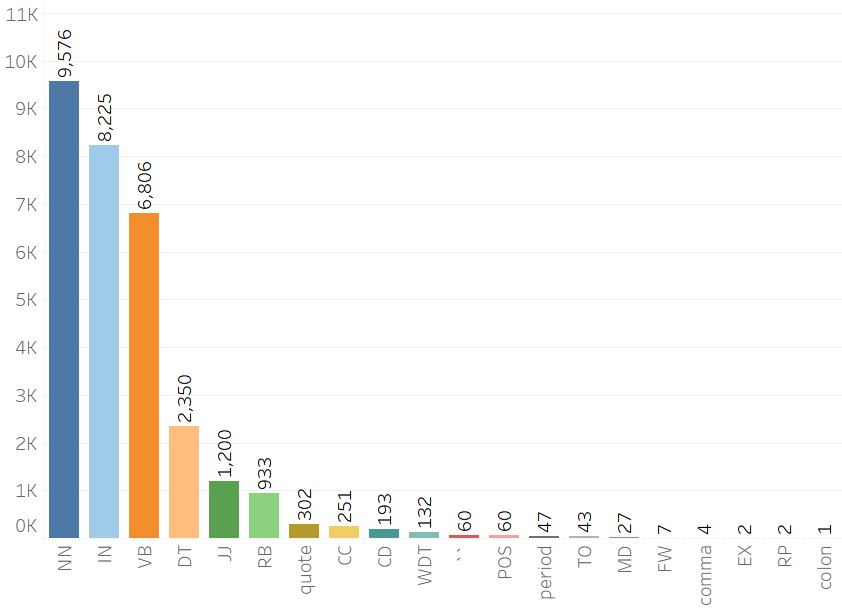
\includegraphics[width=0.95\linewidth]{mainmatter/emnlp2019_delex/histogram_2.jpeg}
    \vspace{-3mm}
    \caption{ Distribution of POS tags that were assigned the highest attention weights by DA for incorrectly classified cross-domain examples.}
  \label{fig:attention}
\vspace{-6mm}
\end{figure}



\subsection{Masking Techniques}\label{masking_techniques}

To mitigate the potential domain dependence introduced by these large attention weights, we propose several semantic masking techniques, which we compare with a deletion baseline.  Examples of each form of masking are shown in Table~\ref{masking_examples}.


\begin{table*}[t]
\begin{center}
\begin{tabular}{p{20mm}|p{55mm}|p{70mm}}

\textbf{Config.} & \textbf{Claim}& \textbf{Evidence} \\ \hline
Lexicalized & {With Singapore Airlines, the Airbus A380 entered commercial service.} & {The A380 made its first flight on 27 April 2005 and entered commercial service on 25 October 2007 with Singapore Airlines.}\\
\hline
NE Deletion & {With  , the  entered commercial service.} & {The A380 made its  flight on  and entered commercial service on  with.}\\
\hline
Basic NER  & {With \texttt{organization}, the \texttt{miscellaneous} entered commercial service.} & {The A380 made its \texttt{ordinal} flight on \texttt{date} and entered commercial service on \texttt{date} with \texttt{organization}.}\\
\hline
OA-NER  & {With \texttt{organization-c1}, the \texttt{misc-c1} entered commercial service.} & {The A380 made its \texttt{ordinal-e1} flight on \texttt{ date-e1} and entered commercial service on \texttt{date-e2} with \texttt{organization-c1}.}\\
\hline

\mbox{OA-NER+SS} Tags & {With \texttt{organization-c1}, the \texttt{artifact-c1} \texttt{motion-c1} commercial \texttt{act-c1} .} & {The A380 \texttt{stative} its \texttt{ordinal-e1 cognition-e1} on \texttt{date-e1 date-e2 date-e3} and \texttt{motion-c1} commercial \texttt{act-c1 on date-e4 date-e5 date-e6} with \texttt{organization-c1}.
}\\

\end{tabular}
\end{center}

    \caption{ Example illustrating our various masking techniques, compared to the original fully lexicalized data. Note that the masking tags were generated with real-world (imperfect) tools. For example, ``Airbus A380" in the claim was correctly classified as \texttt{miscellaneous} by the NER tool, while ``A380" in the evidence was not, thus preventing us from taking advantage of the overlap. }
    \label{masking_examples}
\end{table*}

{\flushleft{\textbf{Named Entity (NE) Deletion Baseline:} }}
Lexical items which are tagged as named or numeric entities (NE) by CoreNLP's named entity recognizer (NER)~\citep{manning2014stanford} are deleted.

{\flushleft{\textbf{Basic NER:}}}  Token sequences which are labeled as NEs are replaced by the corresponding label, e.g., \texttt{location, person}.

{\flushleft{\textbf{Overlap Aware NER (OA-NER)}: }} This technique additionally captures the \textit{lexical overlap} between the claim and evidence sentences with entity ids.
That is, the first instance of a given entity in the claim is tagged with \texttt{c1}, where the \texttt{c} denotes the fact that it was found in the claim sentence (e.g., \texttt{person-c1}). Wherever this {\em same} entity is found later, in claim or in evidence, it is replaced with this unique tag. If an entity is found only in evidence, then it is denoted by an \texttt{e} tag. (e.g., \texttt{location-e3} would be the third location found only in the evidence).

For example, in the claim-evidence pair shown in Table~\ref{masking_examples}, when the named entity \textit{Singapore Airlines} appears in the claim it is replaced with \texttt{organization-c1}, since it is the first \texttt{organization} to appear in claim.
The same id is used wherever the same entity is seen again, e.g., in the evidence sentence. However, the date \textit{27 April 2005} occurs only in the evidence, and hence it is replaced with \texttt{date-e1}.
Importantly, we create pseudo-pretrained embeddings for these new OA-NER-based tokens by adding a small amount of random Gaussian noise (mean 0 and variance of 0.1) to pre-trained embeddings~\citep{pennington2014glove} of the root word corresponding to the category (e.g., \textit{person}). Thus the embeddings of all the sub-tags, while being unique, are close to that of the root word.
{\flushleft{\textbf{OA-NER + Super Sense (SS) Tags}}}:
Super-sense tagging is a sequence modeling approach that annotates phrases with coarse WordNet senses~\citep{ciaramita2003supersense,miller1990introduction}. In this masking method, we not only replace named entities with their OA-NER tags, but also replace other lexical items with their corresponding super sense tags, if found. As with the OA-NER approach, the lexical overlap is also explicitly marked for all these tags with unique ids (see Table~\ref{masking_examples}).


\begin{table*}[ht]
\begin{center}
\begin{tabular}{p{22mm}|p{9mm}p{9mm}p{9mm}p{9mm}}
 & \multicolumn{4}{c}{Configuration} \\
 \hline
Train Domain & {FNC}& {FEVER}  & {FEVER} & {{FNC}} \\
Eval Domain & {FNC}& {{FNC}}  & {FEVER} & {{FEVER}} \\ \hline
Masking & & & & \\
\hline
Lexicalized &96.39\%& {48.86\%} &83.43\%& {41.16\%} \\
%\hline
Deletion  &66.45\%& 40.23\% &75.34\%& 33.33\% \\
%\hline
Basic NER &69.40\%& 46.27\% &76.23\%& 35.72\%\\
%\hline
\textbf{OA-NER} &65.85\%& \textbf{53.59}\% &{82.31\%}& {46.47\%}\\
%\hline
\textbf{OA-NER+SS} & 45.51\%& 46.71\% &75.26\%& {\bf 51.77\%}\\
\end{tabular}
\end{center}
    \caption{\label{crossdomain} Various masking techniques and their performance accuracies, both in-domain and out-of-domain.} \label{tab:results}

\end{table*}
\label{attention_analysis}
We use the word-level attention weights~\citep{bahdanau2014neural} learned by DA to perform  an error analysis in the cross-domain evaluation.
In particular, we first trained two equivalent DA models, one on FEVER and the other on FNC.
Next, we used both models to predict instances in FEVER development. For each data instance, we calculated the cumulative attention weights assigned by each of the two models to all evidence words.
For each of the data instances that were {\em incorrectly} classified by the model trained out of domain (i.e., on FNC) and were {\em correctly} classified by the in-domain model,
we  selected the words that were present in the set of top three words with the highest attention score according to the out-of-domain model, but were {\em not} present in the equivalent set produced by the in-domain model. Such words indicate potential overfitting of the out-of-domain model.
Figure \ref{fig:attention} shows the distribution of part-of-speech (POS) tags for these words. The figure indicates that, for incorrectly classified examples in cross-domain, the higher attention weights were assigned to nouns.
Importantly, 43.10\% of these noun phrases in FEVER are named entities. With this analysis, we are able to confirm that most of the weight is assigned to POS tags of nouns or elements of noun phrases, which confirms our observation that these models anchor themselves on lexical information that is more likely to be domain dependent.

\section{Results and Discussion}
\label{sec:results}

In Table \ref{tab:results} we provide the fact verification results of the state-of-the-art DA model trained with each of our masking approaches, as well as with the original fully lexicalized input.
First, we note that indeed the fully lexicalized model, which performs well in-domain, transfers very poorly to a new domain.
For example, the lexicalized model trained on FEVER,  gave an accuracy of 83.43\% when tested on FEVER, but reduced to 48.86\% when tested on FNC.
This verifies our findings that the signal the model learns from unmasked text does not generalize well.
Additionally, the deletion baseline performs even worse than the fully lexicalized model, which indicates that while the original text can be too domain-specific, its semantic content needs to be maintained on some level.

In terms of this work, we see that all of our masking approaches improve accuracy in the cross-domain setting, by as much as 10.6\% (25.8\% relative), while still maintaining strong in-domain performance (dropping only a few percentage points).
The best cross-domain performance is obtained using our methods which are overlap-aware, suggesting that even when content is abstracted (i.e., masked), the model benefits from explicit awareness of lexical overlap for fact verification. For example, the overlap-aware SS tagging model that was trained on FNC, gave the highest accuracy of 51.77\% when tested out-of-domain, on FEVER.

We note that the model trained on FNC is able to get optimal performance in the FEVER dataset when using the OA-NER + SS tag masking, while the addition of super sense tags did not benefit the model that was trained on FEVER.
This could be due to the fact that overall, the evidence provided in FNC is much longer than that of FEVER,
and perhaps the model needs more training data to learn stable signal from the SS tags.
More importantly, this also suggests that while we have demonstrated that semantic masking is clearly beneficial, it is unclear exactly what level of masking granularity should be employed for a given domain -- from coarse-grained NER tags, to the more granular super sense tags, perhaps even to very fine-grained tags such as those proposed by \citep{ling2012fine}.

\section{Conclusion}

We investigated the importance placed by neural network methods for textual entailment on various lexical items. We concluded that attention weights tend to be directed towards words that are more likely to be domain specific, which
considerably impacts performance in an out-of-domain setting.
To mitigate this issue, we introduced several strategies for semantically masking word classes such as nouns and verbs, by generalizing them to more abstract concepts, which are more likely to have similar usage across domains.
%We also demonstrate the utility of masking named entities for increasing cross-domain performance in RTE tasks.
We demonstrated the utility of our approach in a cross-domain evaluation of textual entailment for fact verification. Our approach outperforms a model trained on the original, fully-lexicalized texts by over 10\% accuracy when evaluated out of domain.
Since our approach is implemented as a data pre-processing step, it can potentially help any neural method that learns from text and is likely to be used out of domain.




\input{mainmatter/emnlp2016-causal/emnlp2016_main}
\input{mainmatter/tacl2015-tig/cl2017_main}
\input{mainmatter/emnlp2017-qaj/emnlp2017_main}
\include{mainmatter/conclusion}
%% Include the various appendices
%\appendix
\include{mainmatter/appendix_rules}

% Switch the spacing to single-spaced for the references
\renewcommand{\baselinestretch}{1}		% changing the value
\small\normalsize										% switch size to make the value take

% Create the References list
\bibliographystyle{uabibnat}
\bibliography{mainmatter/refs}

\end{document}
